% !TEX root = ../main.tex

\chapter{Desarrollo del Proyecto}
\label{ch:otro}

El desarrollo del proyecto se llevó a cabo en tres fases bien diferenciadas, con el objetivo de construir progresivamente una herramienta robusta, funcional y orientada a la experiencia del usuario. A través de una metodología incremental, se fueron implementando las funcionalidades principales desde una primera versión básica hasta llegar a una aplicación completa y adaptativa.

\section{Fase 1: Rectificación Básica}

\textbf{Objetivo:} Implementar la funcionalidad base que permitiera rectificar imágenes de superficies cuadradas a través de transformaciones proyectivas.

\vspace{\baselineskip}

\textbf{Tareas Realizadas:}

\begin{itemize}
    \item \textbf{Creación de la ventana principal:} \\
    Se diseñó una interfaz gráfica básica utilizando la biblioteca \texttt{PySide6}, que permite combinar Python con Qt para el desarrollo de interfaces modernas. Esta ventana principal muestra la imagen cargada por el usuario y permite interactuar con ella. \\
    Para ello, se implementó la clase \texttt{ClickArea}, para gestionar la interacción con la imagen y permitir seleccionar puntos sobre ella mediante clics del ratón.
    
    \item \textbf{Captura y gestión de coordenadas:} \\
    Para estructurar y manipular las coordenadas de manera eficiente, se desarrolló la clase \texttt{Coordinates}. Esta clase encapsula toda la lógica relacionada con el almacenamiento y validación de los puntos seleccionados por el usuario. Entre sus funcionalidades principales se incluye la capacidad de \textbf{almacenar hasta cuatro puntos}, que son aquellos seleccionados mediante clics.
    
    Además, la clase permite \textbf{eliminar un punto} si el usuario hace clic nuevamente sobre él, facilitando la corrección y modificación de la selección. Finalmente, incorpora una \textbf{validación automática} que asegura que se hayan seleccionado exactamente cuatro puntos antes de proceder con la transformación, garantizando así la integridad de los datos para las operaciones posteriores.
    
    
    \item \textbf{Cálculo de los puntos de fuga:} \\
    El cálculo de los puntos de fuga se implementó en el módulo \texttt{infinity\_line.py}, en la función \texttt{calculate\_vanish\_points}. Esta función recibe como entrada cuatro puntos que definen un cuadrilátero sobre la imagen y calcula las intersecciones de los pares de lados opuestos. En concreto, se obtienen dos puntos de fuga mediante la intersección de las siguientes rectas:
    
    \begin{itemize}
        \item La recta que une los puntos $p_1$ y $p_2$ con la que une $p_3$ y $p_4$.
        \item La recta que une los puntos $p_1$ y $p_3$ con la que une $p_2$ y $p_4$.
    \end{itemize}
    
    Estas intersecciones se resuelven mediante álgebra lineal usando la regla de Cramer en \textbf{coordenadas cartesianas}, sin utilizar coordenadas homogéneas. El resultado se devuelve como puntos con $w = 1$, pero los cálculos no son proyectivos en sentido estricto.
        
    Los dos puntos de fuga obtenidos son utilizados posteriormente para definir la recta del infinito en otros módulos. Aunque no se calcula explícitamente la recta proyectiva como producto vectorial (e.g. con \texttt{np.cross(p, q)} en coordenadas homogéneas), esta operación puede incorporarse en el futuro para lograr una interpretación más rigurosa desde la geometría proyectiva.
    
    
    \item \textbf{Transformación proyectiva:} \\
    En el módulo \texttt{projective\_transform.py}, se desarrollaron dos funciones clave:

    \begin{itemize}
        \item \texttt{calculate\_homography}: Calcula la \textbf{matriz de homografía} que permite transformar un cuadrilátero irregular (producto de la perspectiva) en un cuadrado perfecto en la nueva imagen. La función utiliza una base de referencia estándar y resuelve el sistema mediante \textbf{álgebra lineal}.
        
        La homografía se calcula mapeando:
        \begin{itemize}
            \item Los \textbf{puntos de fuga}, obtenidos como intersecciones de lados opuestos del cuadrilátero, a direcciones canónicas \([1, 0, 0]\) y \([0, 1, 0]\).
            \item Dos \textbf{esquinas del cuadrilátero} (específicamente \(p_0\) y \(p_3\)) a posiciones fijas que determinan la escala y orientación del plano rectificado.
        \end{itemize}
        Finalmente, se aplica una \textbf{matriz de escala diagonal} (escalado anisotrópico) para ajustar la \textbf{razón de aspecto} del plano rectificado. Este escalado no representa una transformación afín completa, sino una modificación de la proporción entre ejes horizontal y vertical.
    
        \item \texttt{warp\_perspective\_qpixmap}: Aplica la homografía calculada a la imagen original para obtener una imagen \textbf{rectificada}. Esta función implementa la transformación inversa para cada píxel del plano destino: se aplica la \textbf{inversa de la homografía} para mapear cada píxel en la imagen de salida a su posición correspondiente en la imagen original. Este enfoque evita \textbf{huecos} o \textbf{solapamientos}, al garantizar que cada píxel destino proviene de una ubicación definida en la imagen fuente, pero resulta \textbf{computacionalmente ineficiente} en imágenes de gran tamaño.
    \end{itemize}
    
    \item \textbf{Integración y pruebas:} \\
    Una vez implementadas todas las funciones anteriores, se integraron en el flujo de trabajo principal de la aplicación. El usuario podía:
    \begin{enumerate}
        \item Cargar una imagen.
        \item Seleccionar 4 puntos sobre la imagen.
        \item Hacer clic en el botón “Rectificar”.
    \end{enumerate}
    La aplicación realizaba la transformación y mostraba la imagen corregida. Se llevaron a cabo pruebas con imágenes que contenían superficies cuadradas en distintas perspectivas, confirmando la efectividad de la transformación proyectiva.
\end{itemize}

\section{Fase 2: Adaptación a Otras Proporciones}

\textbf{Objetivo:} Generalizar la herramienta para que pueda rectificar no solo cuadrados, sino también rectángulos con proporciones específicas. Para ello, se añadió la posibilidad de que el usuario introduzca manualmente la razón de aspecto deseada a través de la interfaz gráfica, permitiendo así adaptar la rectificación a cualquier proporción que se requiera.

\vspace{\baselineskip}

\textbf{Tareas Realizadas:}

\begin{itemize}
    \item \textbf{Introducción de la razón de aspecto:} \\
    Se añadió un nuevo widget llamado \texttt{AspectRatioWidget} dentro del archivo \texttt{menu.py}, que permite al usuario introducir manualmente una razón de aspecto (alto/ancho). Esta se utiliza para adaptar la referencia proyectiva a las proporciones deseadas.
    
    \item \textbf{Ajuste de la homografía:} \\
    La función \texttt{calculate\_homography} fue extendida para admitir una razón de aspecto como parámetro adicional. Esta razón permite ajustar la base estándar, originalmente un cuadrado, para transformarla en un rectángulo con las proporciones deseadas.
    
    De este modo, se garantiza que la homografía resultante respete las proporciones especificadas por el usuario. Además, se incorpora un factor de escala que mantiene el tamaño visual coherente dentro de la imagen transformada, asegurando que la rectificación no distorsione la apariencia del resultado final.
    
    \item \textbf{Pruebas con rectángulos:} \\
    Se realizaron múltiples pruebas con diferentes proporciones. Los resultados confirmaron que la herramienta puede adaptarse a una amplia variedad de formatos manteniendo una alta precisión en la rectificación.
\end{itemize}

\section{Fase 3: Interfaz de Usuario}

\textbf{Objetivo:} Mejorar la experiencia del usuario con una interfaz más atractiva, intuitiva y coherente con las convenciones modernas de diseño.

\textbf{Tareas Realizadas:}

\begin{itemize}
    \item \textbf{Diseño de la interfaz:} \\
    Se reestructuró la ventana principal para incluir un menú lateral (\texttt{Menu} en \texttt{menu.py}). Este menú contiene:
    \begin{itemize}
        \item Título de la aplicación con su logo (que puede verse en la Figura~\ref{fg:logo}).
        \item Instrucciones de uso, en un apartado desplegable (apreciable en la Figura~\ref{fg:instructions}).
        \item Campo para introducir la razón de aspecto.
        \item Botones para cargar imagen, aplicar la transformación, borrar todos los puntos seleccionados y descargar la imagen una vez ha sido rectificada.
    \end{itemize}
    
    \begin{figure}[H]
        \centering	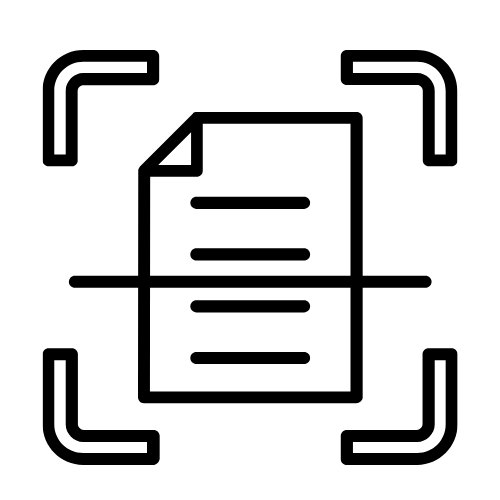
\includegraphics[width=0.2\textwidth]{figures/3.3.LogoDark.png}
        \caption{Logo de la aplicación}\label{fg:logo}
    \end{figure}
    
    \begin{figure}[H]
        \centering	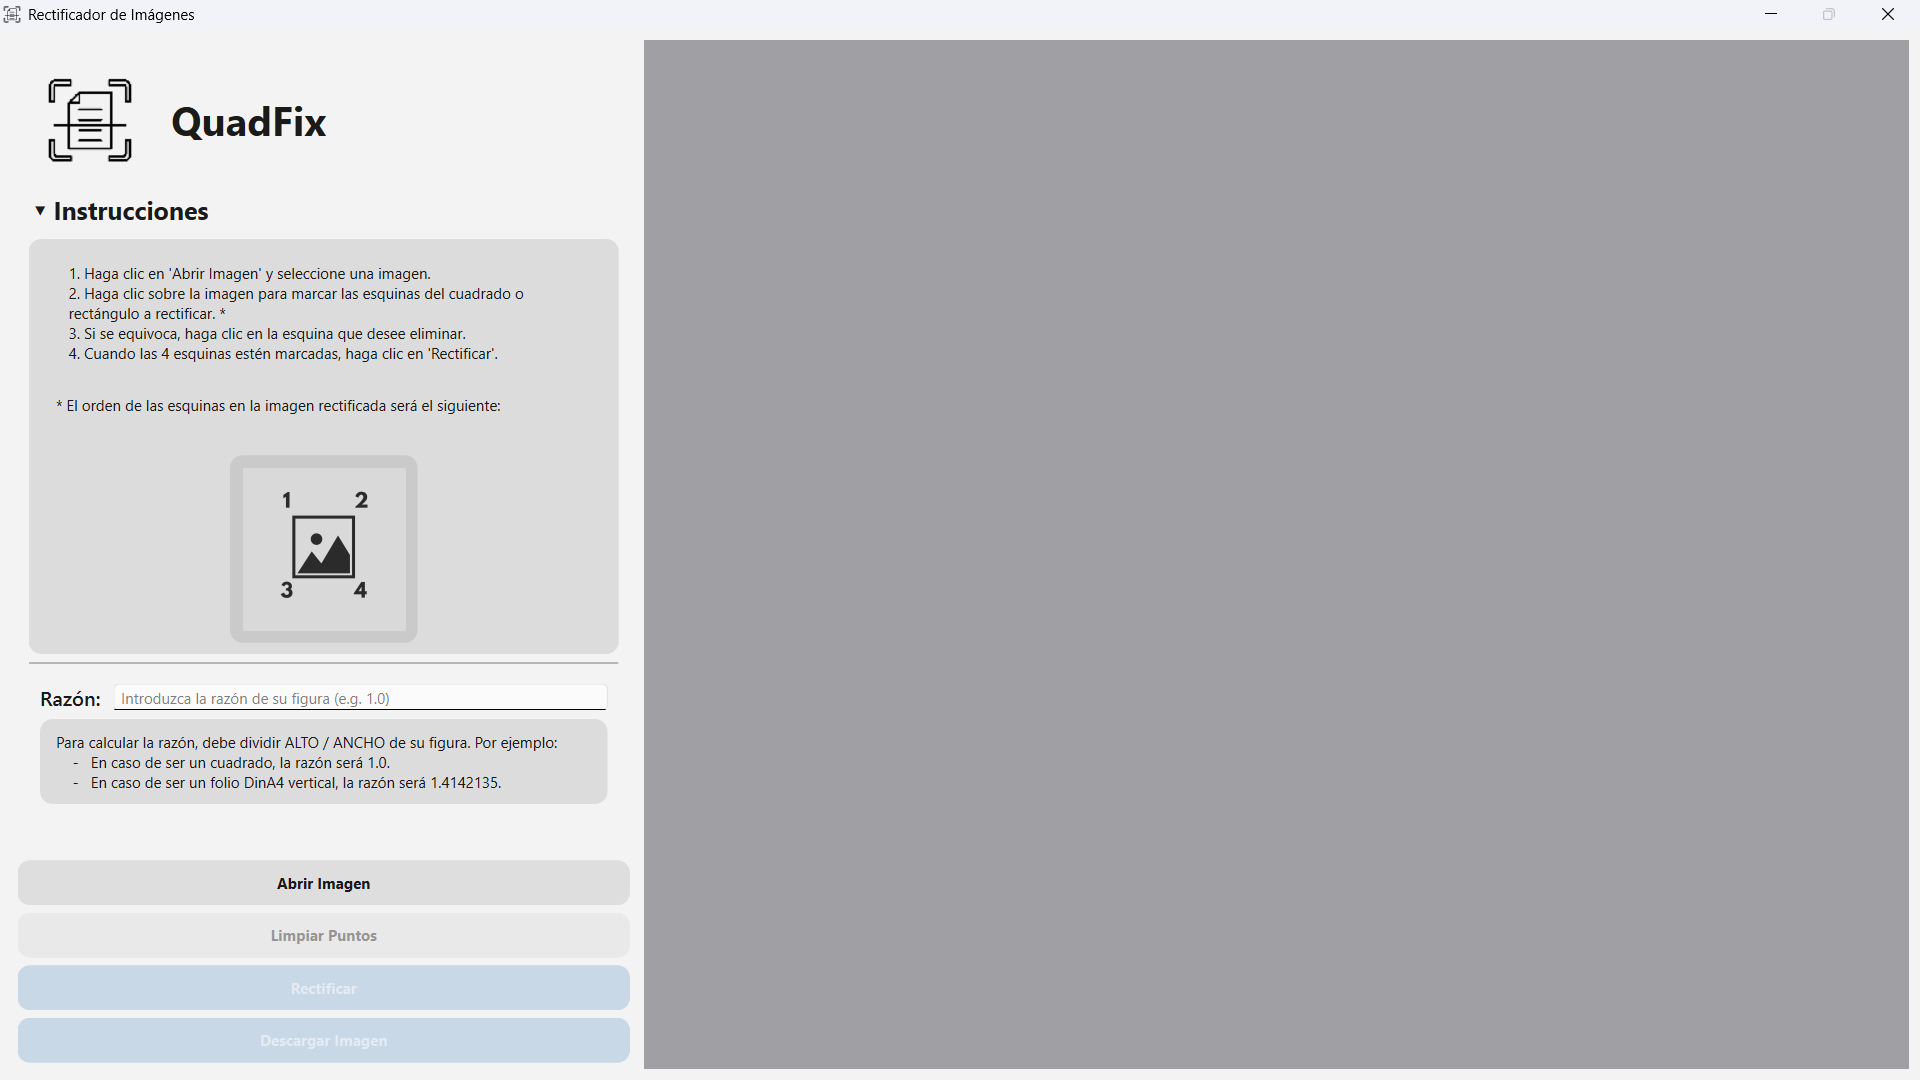
\includegraphics[width=0.8\textwidth]{figures/3.3.Instrucciones.png}
        \caption{Pantalla principal con el apartado ``Instrucciones'' desplegado}\label{fg:instructions}
    \end{figure}
    
    También se definieron dos tipos de botones personalizados, como puede apreciarse en la Figura~\ref{fg:instructions} (\texttt{PrimaryButton}, de color azul, y \texttt{SecondaryButton}, de color negro, en \texttt{buttons.py}) para mejorar la coherencia visual y la jerarquía de acciones.
    
    \item \textbf{Modo claro y oscuro:} \\
    La aplicación detecta el tema del sistema operativo mediante la función \texttt{is\_dark\_mode} (archivo \texttt{dark\_mode.py}) y adapta automáticamente los iconos, los colores del fondo, texto y contenedores y los estilos de los widgets para mantener la legibilidad. En las Figuras ~\ref{fg:light} y \ref{fg:dark} pueden verse los dos modos.

    \begin{figure}[H]
        \centering	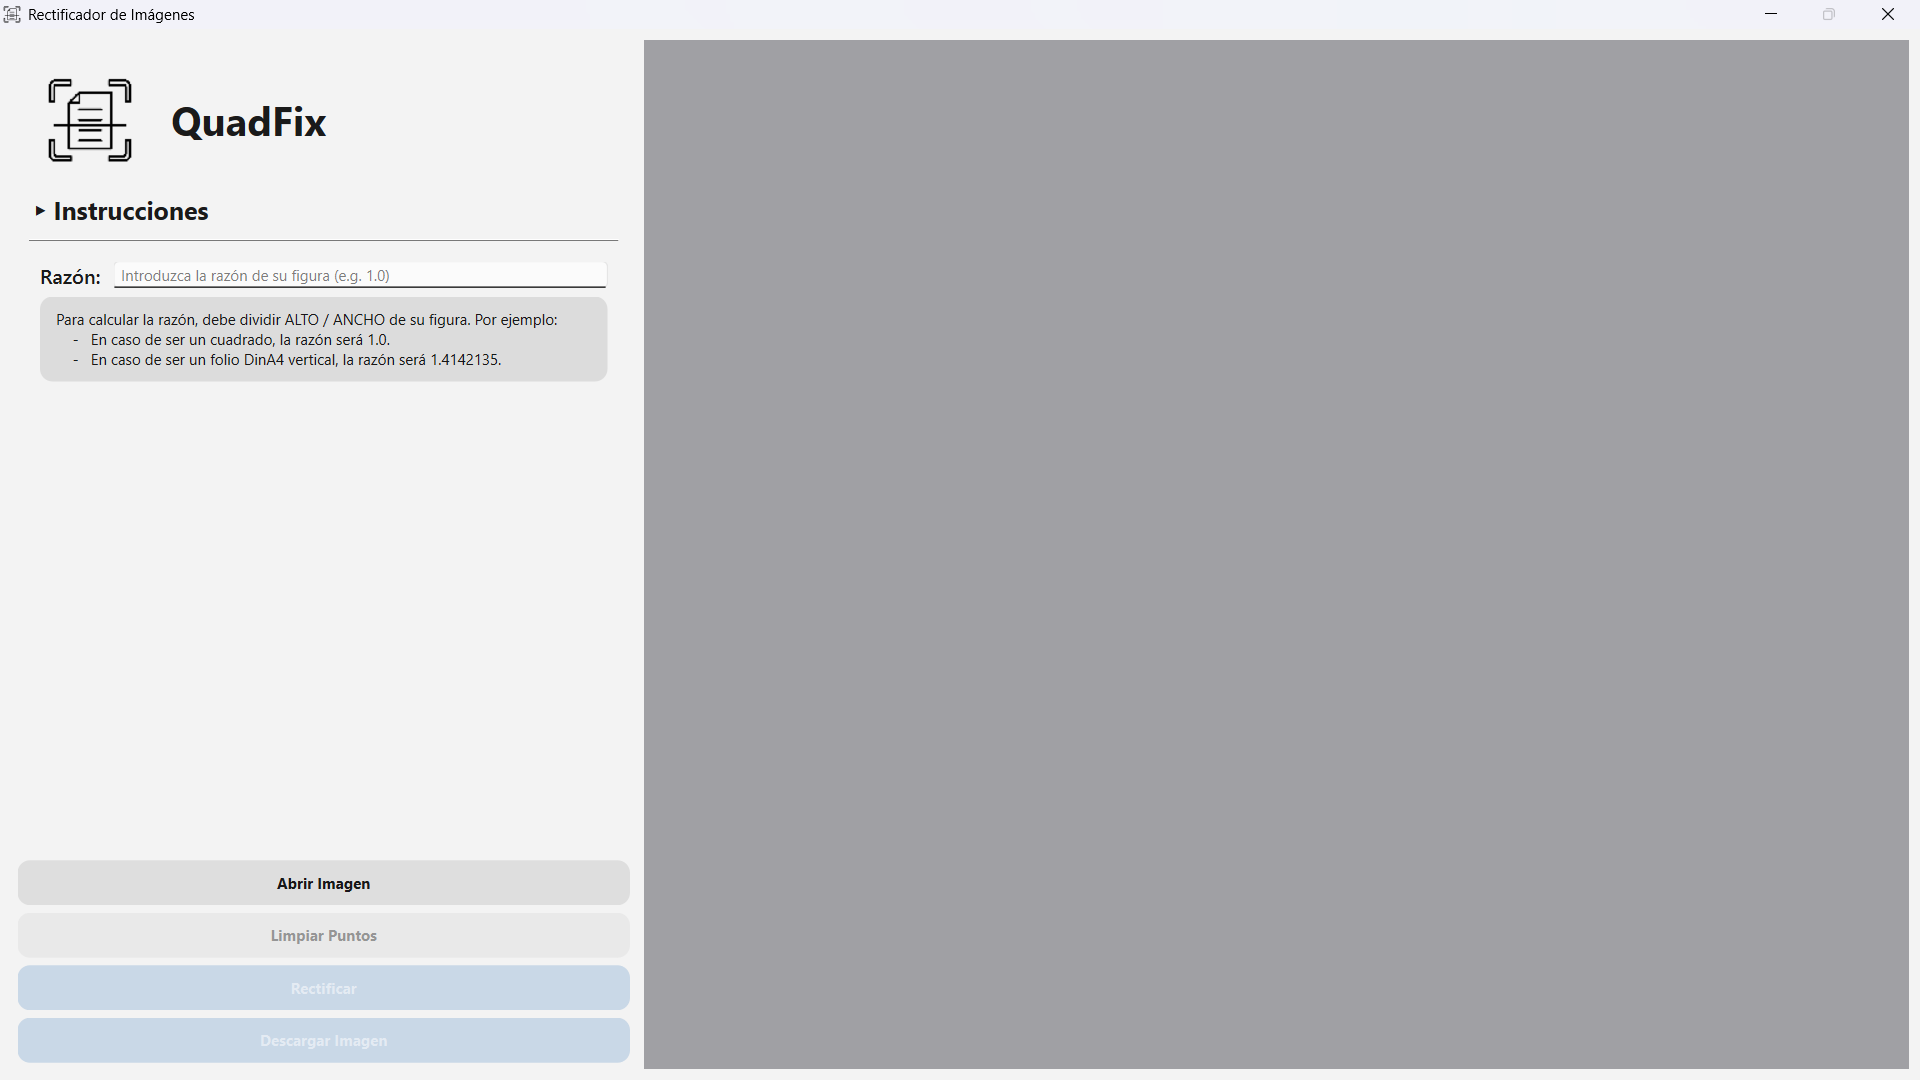
\includegraphics[width=0.65\textwidth]{figures/3.3.Light.png}
        \caption{Modo Claro de la aplicación}\label{fg:light}
    \end{figure}

    \begin{figure}[H]
        \centering	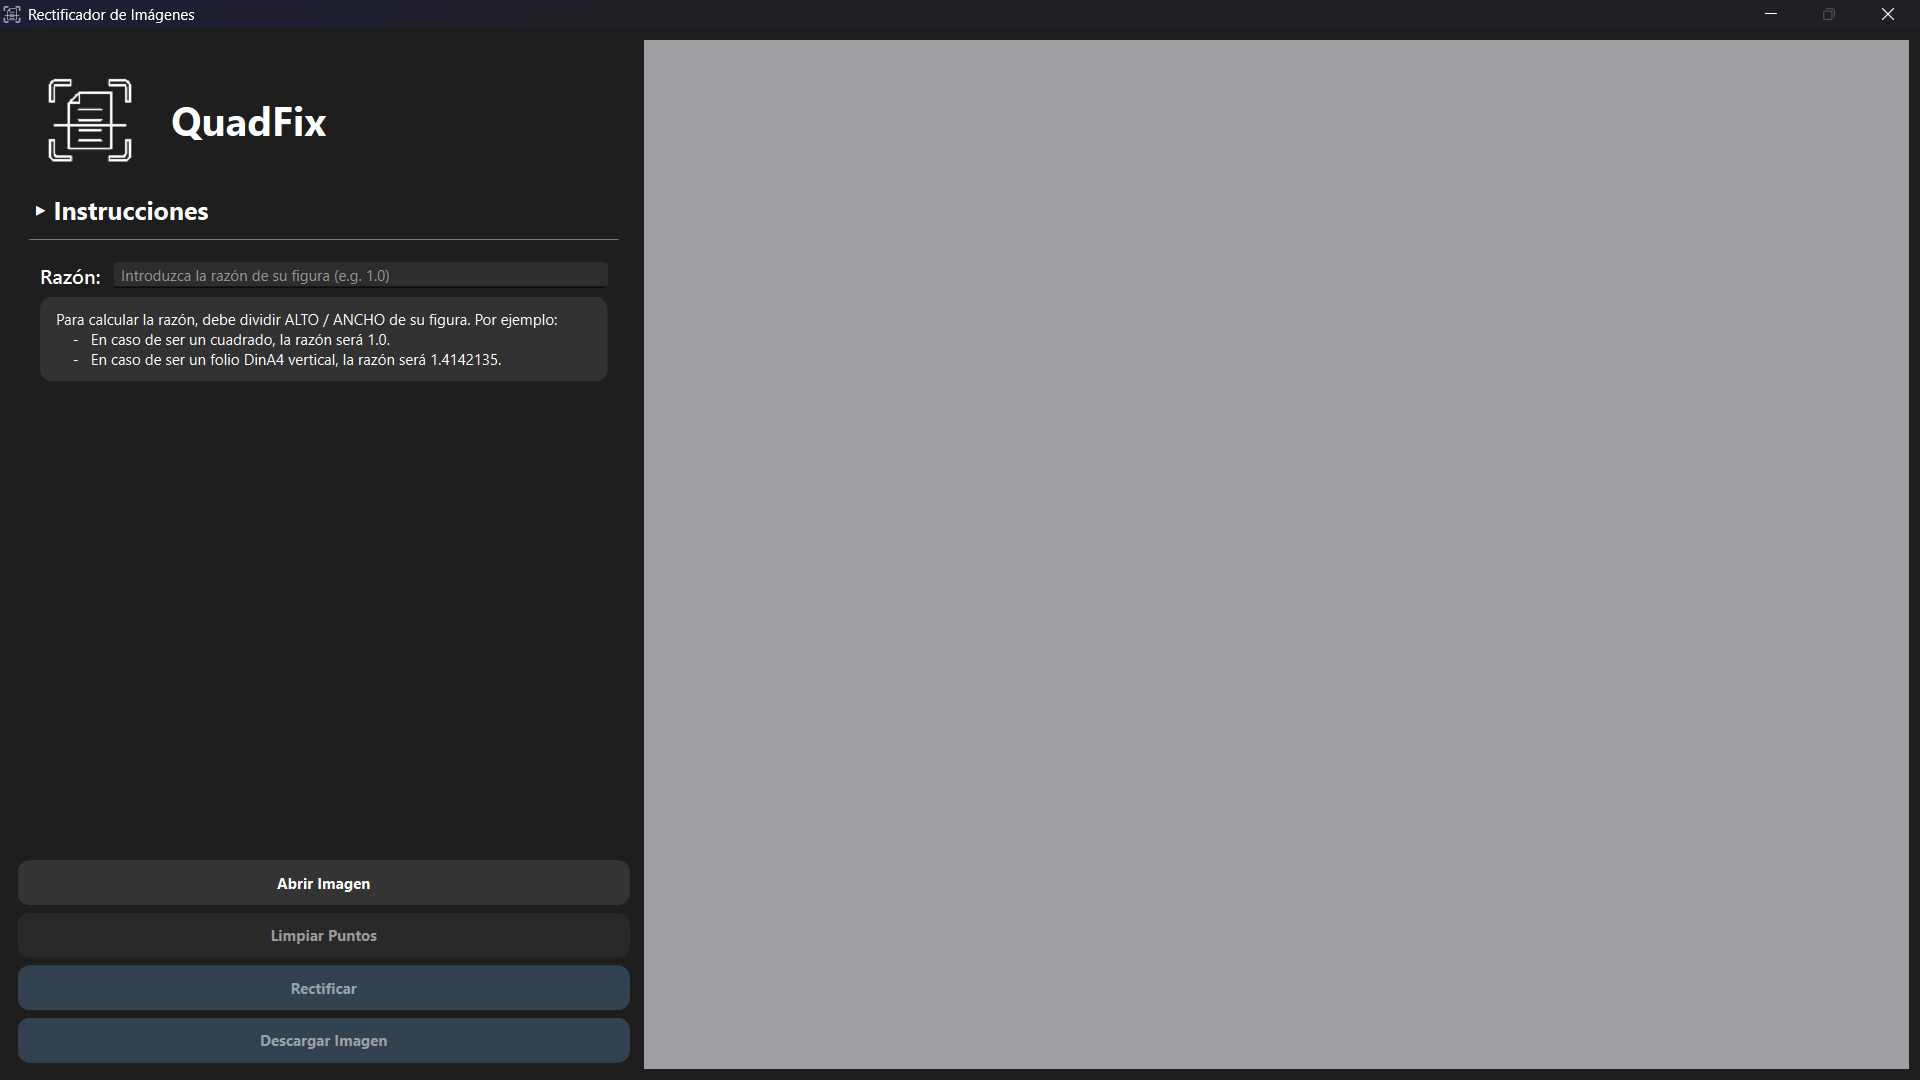
\includegraphics[width=0.65\textwidth]{figures/3.3.Dark.png}
        \caption{Modo Oscuro de la aplicación}\label{fg:dark}
    \end{figure}
    
    \item \textbf{Feedback visual al usuario:} \\
    Se incorporaron diversos mecanismos para mejorar la comunicación con el usuario durante la interacción con la aplicación. Entre estos, destaca un \textit{widget} de carga, implementado como \texttt{OverlayWidget} en el módulo \texttt{click\_area.py}, que se muestra mientras la imagen está siendo procesada.
    
    Además, se añadieron mensajes de error que alertan al usuario en caso de que el número de puntos seleccionados sea incorrecto, si la imagen no ha sido cargada correctamente, o si la descarga de la imagen no ha podido completarse. Por último, se implementaron confirmaciones visuales que informan al usuario sobre el éxito de las transformaciones realizadas o la descarga correcta de la imagen.
    
    \item \textbf{Optimización y detalles finales:} \\
    Se ajustaron los márgenes, tipografías, colores y alineaciones para garantizar un diseño limpio y profesional. Además, se añadió una función para guardar la imagen rectificada en el sistema del usuario, mejorando la utilidad práctica de la herramienta.
\end{itemize}

\section{Conclusión del Desarrollo}

A lo largo de las tres fases, el proyecto evolucionó desde una funcionalidad básica centrada en la geometría proyectiva hasta convertirse en una aplicación visualmente pulida, práctica y adaptable a distintos contextos. Cada fase aportó un avance significativo:

\begin{itemize}
    \item \textbf{Fase 1:} Estableció las bases matemáticas y funcionales.
    \item \textbf{Fase 2:} Amplió la versatilidad con soporte para diferentes formatos.
    \item \textbf{Fase 3:} Cerró el desarrollo con una interfaz moderna y experiencia de usuario cuidada.
\end{itemize}

El resultado final es una herramienta que combina precisión matemática con una usabilidad óptima, apta para tareas de corrección de perspectiva en distintos formatos de imagen.
